\documentclass[12pt,a4paper]{article}
\usepackage[utf8x]{inputenc}
\usepackage{ucs}
\usepackage[finnish]{babel}
\usepackage[T1]{fontenc}
\usepackage{amsmath}
\usepackage{amsfonts}
\usepackage{amssymb}
\usepackage{graphicx}
\usepackage{hyperref}
\usepackage[figurename=Kuva, tablename=Taulukko]{caption}

\author{Vesa Hagström}


\begin{document}
    \renewcommand{\bibname}{Viitteet}

	\begin{titlepage}
    \label{Title}
	\begin{flushleft}
		\hfill Vesa Hagström 											\\
		\hfill \texttt{vesa.hagstrom@helsinki.fi} 						\\
		\hfill Op.Nro: 013865575											\\
		\hfill Tiralabra harjoitustyö									\\
		\hfill 16.6.2013													\\
	\end{flushleft}

	\vfill

	\begin{center}
		\huge{Simrec toteutusdokumentti}
	\end{center}

	\vfill

	\end{titlepage}

    \section{Ohjelman yleisrakenne}
        Simrec koostuu kahdesta luokasta ja kahdesta nimiavaruudesta, mitkä kaikki sisältyvät \textit{simrec} nimiavaruuteen. Ohjelman algoritmit sijaitsevat nimiavaruudessa \textit{simrec::algorithms} ja muuten hyödylliset funktiot ja vakiot -- kuten $\pi$ -- \textit{simrec::utils}:sta. 
        
        Data säilytetään yksinkertaisissa tietorakenteissa \textit{Image} ja \textit{ComplexArray}. \textit{Image} tietorakenne on toteutettu \textit{ComplexArray}:lla, eli \textit{Image} on käytännössä vain kaksiulotteinen \textit{ComplexArray}. 
        
        Ohjelman rakenne on kuvattu UML luokkakaaviossa kuvassa (\ref{uml}).
        
	    \begin{figure}
		\noindent\makebox[\textwidth]{%
		    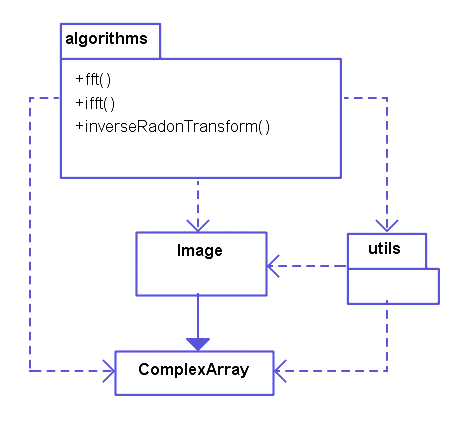
\includegraphics[width=1.2\textwidth]{luokkakaavio}
		}
		\caption{Simrec:n UML luokkakaavio}
	    \label{uml}
		\end{figure}
    
        Ohjelmaan siis luetaan kuvadata, mikä tallennetaan kompleksilukuina \textit{ComplexArray}-olioon. Tämän olion ja kuvan dimensioiden perusteella luodaan \textit{Image}-olio. \textit{Image}-olion avulla data skaalataan FFT-algoritmille sopivaan kokoon, eli sellaiseksi, että sen sivut ovat pituudeltaan pienin kahden potenssi, mikä on suurempi kuin kuvan pidemmän sivun pituus. Tämän jälkeen \textit{Image}-olion data Fourier-muunnetaan, filtteröidään ja Fourier-käänteismuunnetaan \textit{simrec::algorithms}:ssa sijaitsevilla algoritmeilla. Tämä filtteröity data sitten Radon-käänteismuunnetaan \textit{simrec::algorithms}:n sisältämällä algoritmilla.
        
    \section{Saavutetut aika- ja tilavaativuudet}
    Kuvadatan filtteröinnissä käytettävän Fourier-muunnoksen ja Fourier-käänteismuunnoksen aikavaativuudet algoritmista analysoituna ovat molemmat $O(n \log n)$, kuten FFT:n olettaisikin olevan. 2D FFT:ssä suoritetaan myös kaksi kuvamatriisin transponointioperaatiota, joiden aikavaativuudet ovat $O(\frac{n}{2}) \approx O(n)$. Kuvalle suoritettavat filtteröinnit ovet aikavaativuudeltaan $O(n)$, sillä niissä käydään koko kuvadata läpi kertaalleen. Radon-käänteismuunnos on aikavaativuudeltaan luokkaa $O(n^3)$.  \\
    Näistä laskemalla $O(2 \cdot n \log n + n + n + n^3) \approx O(n^3)$. Algoritmin ajamiseen kuluva aika eri syötteko'oilla näkyy mitattuna kuvassa (\ref{kuvaaja}). 
    
     Ohjelma tallentaa muistiin tiedostosta luetun kuvan, minkä tilavaativuus on $O(n)$. FFT ja iFFT pitävät ajonsa aikana muistissa palasia datasta, ja tilavaativuus näissä on sama kuin FFT:n/iFFT:n aikavaativuus, eli $O(n \log n)$. Radon-käänteismuunnos luo syötedatan koosta riippuvan uuden kuvan, minkä tilavaativuus on siis $O(n)$. Lopullinen tilavaativuus on siis laskettuna $O(n \log n + n + n) \approx O(n \log n)$.

	    \begin{figure}
		\noindent\makebox[\textwidth]{%
		    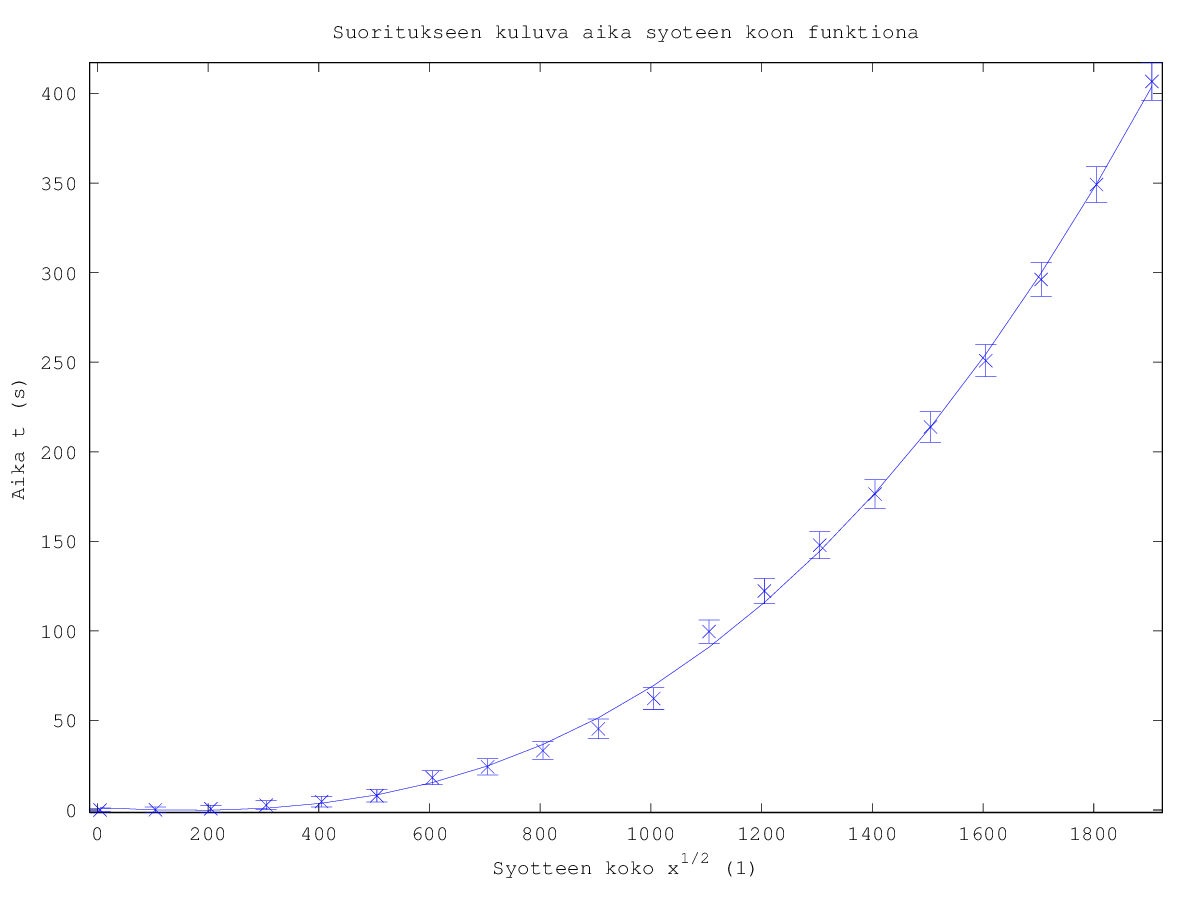
\includegraphics[width=1.2\textwidth]{kuvaaja}
		}
		\caption{Mitatatut ajat eri kokoisilla syötteillä. x=1000 tarkoittaa, että algoritmi ajettiin kuvalla, minkä koko on $1000 \cdot 1000$.}
	    \label{kuvaaja}
		\end{figure}
		 
    \section{Puutteet ja parannusehdotukset}
     Ohjelman algoritmeja voisi optimoida huomattavasti. Esimerkiksi Fourier-muunnoksien $e^{\pm 2 \pi i A}$ -muotoiset kertoimet voisi laskea kerran etukäteen, minkä jälkeen niitä ei tarvitsisi laskea jokaisella FFT:n kierroksella erikseen. Tällä hetkellä algoritmeille myös kopioidaan kussakin kohdassa tarvittavan data (esim. 2D FFT:ssä kuvan rivit) kokonaisdatasta ja suoritetaan algoritmi tälle osalle, minkä jälkeen se syötetään takaisin alkuperäiseen paikkaansa. Tällä hetkellä algoritmit on toteutettu näin, koska se selkeyttää ohjelman rakennetta hieman. 
     
    \newpage

    \begin{thebibliography}{6}
        \bibitem{radonmuunnos}
	    Peter Toft, 
	    \emph{"The Radon Transform - Theory and Implementation"},\\
        	\url{http://petertoft.dk/PhD/}
        	
        	\bibitem{fft}
	    J.W. Cooley, J.W. Tukey 
	    \emph{"An algorithm for the machine calculation of complex Fourier series"},\\
        	\url{http://dx.doi.org/10.1090/S0025-5718-1965-0178586-1}
    \end{thebibliography}
\end{document}